\section{Method}
\label{sec:method}

\subsection{System Overview}
\label{sec:overview}

The system has three stages, shown in Figure~\ref{fig:pipeline}. The first stage accepts a
document and its metadata. The second stage runs a classifier that proposes a topic label
and a confidence score, and a claim extractor that returns the text spans supporting the
label. The third stage routes low-confidence or evidence-poor items to a human reviewer.
The reviewer can accept, edit or reject the proposal, and every action is written to the
audit trail.

\begin{figure}[htbp]
  \centering
  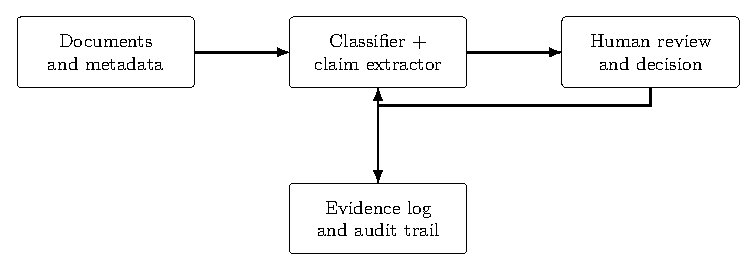
\includegraphics[width=0.86\textwidth]{figures/example-figure.pdf}
  \caption{The three-stage human-in-the-loop triage workflow. Low-confidence items go to
  human review; review actions and evidence are written to the audit trail.}
  \label{fig:pipeline}
  \figsource{Author's own diagram; the division of labour is described in
  Section~\ref{sec:division}.}
\end{figure}

\subsection{Data and the Division of Labour}
\label{sec:division}

The evaluation uses a small synthetic corpus: 48 documents covering two topics, each with a
human-labelled topic. The corpus contains no real student, partner or personal information.
That makes the evaluation safe to publish, and it is also a limit of the prototype.

The division of labour follows one rule: the model proposes, the human decides. The model
only emits a label, a confidence score and evidence spans; it never rejects a document on
its own. Items with confidence below 0.8, or with no evidence span, must go to human review.
The reviewer's final label is the only label written to the official record; the model output
is retained only as a proposal.
